It has been seen in the previous section that the complete solution of a Riemann problems in solid dynamics is possible for simple problems. However, such a solution may become complicated for multi-dimensional problems or for other non-linear problems. 
Numerical methods such as Finite Volume Methods \cite{Leveque} require the solution of many Riemann problems within a discretized medium. When dealing with non-linear problems, the exact solution of those problems may increase drastically the computational cost, making the numerical scheme prohibitive. Moreover, numerical procedures often require only little information about the solution of Riemann problems and do not need the complete resolution. In that context, alternative procedures have been developed in order to take into account the characteristic structure of a hyperbolic system by computing an approximate solution of Riemann problems. Approximate Riemann solvers developed for Computational Fluid Dynamics allow to extract information for either flux functions (\textit{HLL, HLLC, Roe} and \textit{Osher} approximate Riemann solvers \cite{Trangenstein}, \cite{Toro}) or for vectors of conserved quantities (\textit{approximate--state Riemann solver} \cite[Ch.9]{Toro}, \cite[Ch.22]{Leveque}). Some of those have been applied to specific problems in solid mechanics problems such as the Osher approximate solver (see \cite{LEE_FVM} and \cite{Haider_FVM}) or the HLLC approximate solver (see \cite{Ortega_HLLD}) for hyperelasticity . We recall here the formulation of the approximate-state Riemann solver for solid mechanics. The approach is then applied to the non-linear problem of section \ref{subsec:charac_nonlinear_problems}.

\subsection{General ideas}
As in the previous section, we consider the Riemann problem in the space direction $\vect{N}$:
\begin{equation}
  \label{eq:RP_approx}
  \begin{aligned}
  &\Qcb_t + \Jbsf\(\Qcb\) \drond{\Qcb}{X_N} = \vect{0}, \\
  &\left\lbrace 
    \begin{aligned}
      & \Qcb(X_N,t=0) = \Qcb^L \quad \text{if } X_N< 0\\
      & \Qcb(X_N,t=0) = \Qcb^R \quad \text{if } X_N> 0
    \end{aligned}
    \right.
  \end{aligned}
\end{equation}
The approach for developing an approximate-state Riemann solver consists in linearizing the problem \eqref{eq:RP_approx} by approximating $\Jbsf$ in the vicinity of $\Qcb^L$ and $\Qcb^R$ by a constant matrix $\bar{\Jbsf}=\Jbsf\(\Qcb^L,\Qcb^R\)$ \cite[Ch.15]{Leveque}. Note that this approximation is valid for small jumps in initial data (\textit{i.e }$\Qcb^L\approx\Qcb^R$) and that $\bar{\Jbsf}$ must ensure hyperbolicity of the system, namely $\bar{\Jbsf}$ has real eigenvalues and a complete set of independent eigenvectors. The approximate matrix also satisfies the consistency condition:
\begin{equation}
  \label{eq:approx_constistency}
  \bar{\Jbsf}\(\Qcb,\Qcb\)=\Jbsf\(\Qcb\)
\end{equation}

Such a matrix can be defined by using the definition of right eigenvectors and characteristic speeds $\Jbsf \Rbsf = \Rbsf \Cbsf \Rightarrow \Jbsf = \Rbsf \Cbsf \Rbsf^{-1}$ in which left-going (\textit{resp. right-going}) characteristics and associated eigenvectors are assumed to depend on $\Qcb^L$ (\textit{resp. on} $\Qcb^R$) only. Namely, one writes:
\begin{align*}
  &\Rbsf = \matrice{\Rcb^1(\Qcb^L),\cdots,\Rcb^I(\Qcb^L),\Rcb^{I+1}(\Qcb^R),\cdots,\Rcb^m(\Qcb^R)} \\
  &\Cbsf=\matrice{c_1(\Qcb^L) & & & & & \\ & \cdots & & && \\ & &c_I(\Qcb^L) & & &\\ & & &c_{I+1}(\Qcb^R)& & \\ & & & &\cdots &\\ &&&&&c_m(\Qcb^R)} 
\end{align*}
where $c_I(\Qcb)$ and $m$ are the highest negative eigenvalue and the dimension of the Jacobian matrix. 

At last, the linearized Riemann problem thus written enables the determination of every state vectors $\Qcb(x,t)$ by following the procedure described in section \ref{subsec:charac_Linear_problems} for linear problems, recalled here for convenience for a system of dimension $m$:
\begin{equation}
  \label{eq:approx_RS}
  \begin{aligned}
    &  \Qcb^R-\Qcb^L=\sum_{i=1}^{m} \Rcb^i\delta^i \\
    &  \Qcb(x,t) =\Qcb^R -\sum_{i=I+1}^{m} \Rcb^i\delta^i \\
    &  \Qcb(x,t) =\Qcb^L+ \sum_{i=1}^{I} \Rcb^i\delta^i
  \end{aligned}
\end{equation}
where the point ($x,t$) lies in the region bounded by the $I$th and $I+1$th characteristics.

\begin{remark}
  Note that since one can define a complete set of independent eigenvectors of the Jacobian matrix, the matrix $\Rbsf$ is non-singular so that $\bar{\Jbsf}$ can be uniquely determined. Moreover, the linearization proposed amounts to considering a heterogeneous medium where $\Qcb^{L}$ and $\Qcb^R$ act as material parameters.
\end{remark}

\subsection{Application: Hyperelastic plane wave}
We finish this section with an illustration of the approximate Riemann solver by considering the plane wave problem in a Saint-Venant-Kirchhoff of section \ref{subsec:charac_nonlinear_problems}.
Recall that the eigenvalues and right eigenvectors matrices read for that problem:
\begin{equation}
  \label{eq:SVK_matrices}
  \Cbsf = \matrice{-c & 0 \\ 0 & c} \quad ; \quad \Rbsf = \matrice{c & -c\\ 1&1} \:,\quad c=\sqrt{\frac{\lambda + 2\mu}{2\rho_0}(3F^2-1)}
\end{equation}
Hence, the linearized problem is written with:
\begin{equation}
  \label{eq:SVK_matrices_linear}
  \Cbsf = \matrice{-c_L & 0 \\ 0 & c_R} \quad ; \quad \Rbsf = \matrice{c_L & -c_R\\ 1&1}
\end{equation}
In section \ref{subsec:charac_Linear_problems}, the expression of the wave strengths vector $\vect{\delta}$ has been established for general linear systems of dimension $2$ (see equation \eqref{eq:wave_strengths}):
\begin{equation}
  \vect{\delta}=\frac{1}{c_R+c_L}\matrice{c_R \Delta F +\Delta v\\ c_L \Delta F -\Delta v}
\end{equation}
leading to the solution $\Qcb $ between the two discontinuous waves:
\begin{equation}
  \label{eq:SVK_approx_solution}
  \Qcb  = \Qcb^L + \delta^1 \Rcb^1 = \matrice{v_L \\F_L} +\delta^1 \matrice{c_L \\1} \quad \text{or} \quad \Qcb  = \Qcb^R - \delta^2 \Rcb^2 = \matrice{v_R \\F_R} -\delta^2 \matrice{-c_R \\1}
\end{equation}
Substitutions of $\delta^{1,2}$ from second equations in first ones provide straight lines equations in the phase plane ($F,v$):
\begin{equation}
  \label{eq:approx_straight}
  v  = v_L + c_L(F -F_L) \quad ; \quad v  = v_R + c_R(F_R-F )
\end{equation}
\begin{figure}[h!]
  \centering
  {\definecolor{Purple}{RGB}{120,28,129}
\definecolor{Blue}{RGB}{63,96,174}
\definecolor{Duck}{RGB}{83,158,182}
\definecolor{Green}{RGB}{109,179,136}
\definecolor{Yellow}{RGB}{202,184,67}
\definecolor{Orange}{RGB}{231,133,50}
\definecolor{Red}{RGB}{217,33,32}
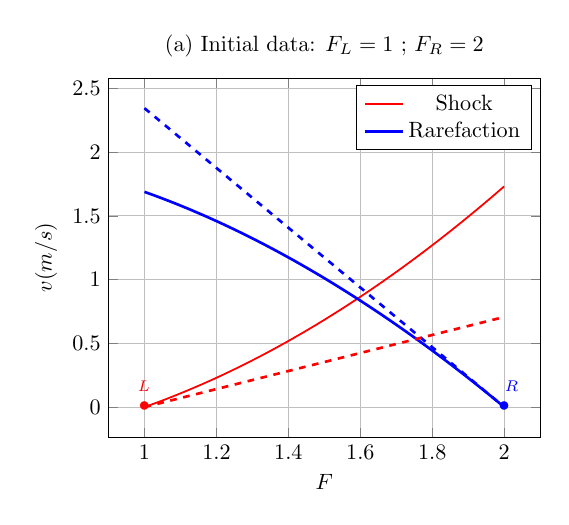
\begin{tikzpicture}[scale=0.8]
\begin{axis}[xlabel=$F$,ylabel=$v (m/s)$,ymajorgrids=true,xmajorgrids=true, title={(a) Initial data: $F_L=1$ ; $F_R=2$}]
  \addplot[Red,thick] coordinates {(1.0,0.0) (1.0196019601960196,0.019889905868838792) (1.0392039203920391,0.04035480171519238) (1.058805880588059,0.06139339246981025) (1.0784078407840785,0.08300445472552491) (1.098009800980098,0.1051868317293367) (1.1176117611761176,0.1279394287977403) (1.1372137213721372,0.1512612091133456) (1.1568156815681567,0.17515118986560513) (1.1764176417641765,0.19960843870261852) (1.196019601960196,0.2246320704646163) (1.2156215621562156,0.25022124417291264) (1.2352235223522352,0.2763751602509047) (1.2548254825482548,0.30309305795616337) (1.2744274427442743,0.330374213004825) (1.2940294029402941,0.3582179353714115) (1.3136313631363137,0.386623567248899) (1.3332333233323332,0.4155904811553686) (1.3528352835283528,0.445118078174895) (1.3724372437243724,0.47520578632153143) (1.3920392039203922,0.5058530590163028) (1.4116411641164117,0.5370593736680643) (1.4312431243124313,0.568824230349938) (1.4508450845084508,0.6011471505637854) (1.4704470447044704,0.6340276760858663) (1.4900490049004902,0.667465367887438) (1.5096509650965095,0.7014598051246006) (1.5292529252925293,0.7360105841921958) (1.5488548854885489,0.7711173178369951) (1.5684568456845684,0.8067796343258441) (1.5880588058805882,0.8429971766647708) (1.6076607660766076,0.8797696018654025) (1.6272627262726274,0.917096580255355) (1.646864686468647,0.9549777948294852) (1.6664666466646665,0.9934129406392047) (1.686068606860686,1.032401724217221) (1.7056705670567056,1.0719438630353144) (1.7252725272527254,1.1120390849929296) (1.7448744874487447,1.1526871279345328) (1.7644764476447645,1.1938877391938512) (1.784078407840784,1.2356406751632294) (1.8036803680368036,1.2779457008865038) (1.8232823282328234,1.320802589673878) (1.8428842884288428,1.3642111227374165) (1.8624862486248626,1.4081710888458763) (1.8820882088208821,1.4526822839976499) (1.9016901690169017,1.4977445111107466) (1.9212921292129215,1.543357579728744) (1.9408940894089408,1.5895213057417645) (1.9604960496049606,1.6362355111215798) (1.9800980098009802,1.6835000236699957) (1.9996999699969997,1.7313146767797576) };
  \addplot[Blue,very thick] coordinates {(1.0,1.6884673989302577) (1.0196019601960196,1.6685781823289632) (1.0392039203920391,1.648117983645035) (1.058805880588059,1.6270917763366024) (1.0784078407840785,1.6055041425368688) (1.098009800980098,1.5833593157699348) (1.1176117611761176,1.5606612177002648) (1.1372137213721372,1.5374134899261505) (1.1568156815681567,1.5136195216278194) (1.1764176417641765,1.48928247372591) (1.196019601960196,1.4644053000848238) (1.2156215621562156,1.4389907661996928) (1.2352235223522352,1.4130414657294894) (1.2548254825482548,1.3865598351776642) (1.2744274427442743,1.3595481669723095) (1.2940294029402941,1.3320086211576845) (1.3136313631363137,1.3039432358761032) (1.3332333233323332,1.2753539367920979) (1.3528352835283528,1.246242545588463) (1.3724372437243724,1.216610787645106) (1.3920392039203922,1.1864602989961286) (1.4116411641164117,1.1557926326474621) (1.4312431243124313,1.12460926432638) (1.4508450845084508,1.092911597724879) (1.4704470447044704,1.0607009692909792) (1.4900490049004902,1.0279786526152188) (1.5096509650965095,0.994745862453826) (1.5292529252925293,0.9610037584250569) (1.5488548854885489,0.9267534484108921) (1.5684568456845684,0.8919959916925568) (1.5880588058805882,0.8567324018451127) (1.6076607660766076,0.8209636494135533) (1.6272627262726274,0.7846906643903794) (1.646864686468647,0.7479143385125069) (1.6664666466646665,0.7106355273934435) (1.686068606860686,0.6728550525050632) (1.7056705670567056,0.6345737030218022) (1.7252725272527254,0.595792237538853) (1.7448744874487447,0.5565113856747698) (1.7644764476447645,0.5167318495678894) (1.784078407840784,0.47645430527509447) (1.8036803680368036,0.43567940408061234) (1.8232823282328234,0.3944077737218566) (1.8428842884288428,0.3526400195386741) (1.8624862486248626,0.31037672555176576) (1.8820882088208821,0.2676184554755838) (1.9016901690169017,0.22436575367049583) (1.9212921292129215,0.18061914603862234) (1.9408940894089408,0.13637914086738703) (1.9604960496049606,0.09164622962443836) (1.9800980098009802,0.04642088770736517) (1.9996999699969997,0.0007035751512764867) };
  \node at (axis cs:1,0) [Red] {$\bullet$};
  \node at (axis cs:2.,0) [Blue] {$\bullet$};
  \node at (axis cs:1,0) [anchor=south,Red] {$\Qcb^L$};
  \node at (axis cs:1.98,0) [above right,Blue] {$\Qcb^R$};
  \addplot[Blue,dashed,very thick,domain=1:2,samples=51,samples y=0]
    ({x},{0.-sqrt(0.5*(12.-1))*(x-2.)});
  \addplot[Red,dashed,very thick,domain=1:2,samples=51,samples y=0]
    ({x},{0.+sqrt(0.5*(2.-1))*(x-1.)});
  \legend{Shock,Rarefaction}
\end{axis}
\end{tikzpicture}
 \phantomsubcaption \label{subfig:SVK_Approx1}}
  {\definecolor{Red}{RGB}{217,33,32}
\definecolor{Blue}{RGB}{63,96,174}
\definecolor{Duck}{RGB}{83,158,182}
\definecolor{Green}{RGB}{109,179,136}
\definecolor{Yellow}{RGB}{202,184,67}
\definecolor{Orange}{RGB}{231,133,50}
\definecolor{Purple}{RGB}{120,28,129}
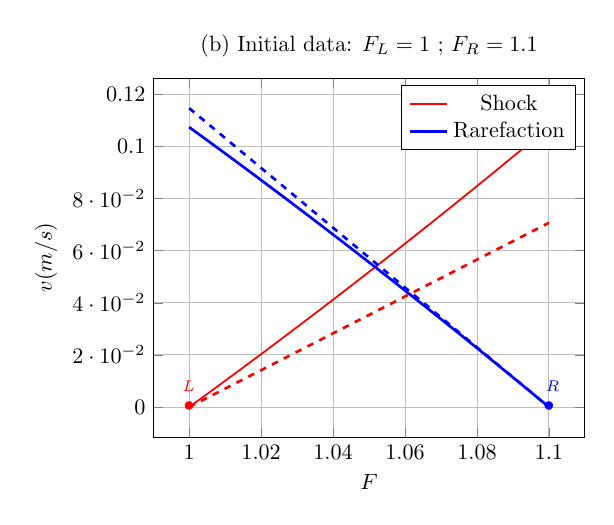
\begin{tikzpicture}[scale=0.8]
\begin{axis}[xlabel=$F$,ylabel=$v (m/s)$,ymajorgrids=true,xmajorgrids=true,title={(b) Initial data: $F_L=1$ ; $F_R=1.1$}]
\addplot[Red,thick] coordinates {(1.0,0.0) (1.001960196019602,0.0019630775609053948) (1.003920392039204,0.003931917267080632) (1.005880588058806,0.005906517718693416) (1.0078407840784078,0.007886877524091035) (1.00980098009801,0.009872995299740863) (1.0117611761176117,0.011864869670167599) (1.0137213721372138,0.01386249926789511) (1.0156815681568157,0.01586588273338493) (1.0176417641764177,0.01787501871497885) (1.0196019601960196,0.019889905868838792) (1.0215621562156216,0.02191054285889049) (1.0235223522352235,0.023936928356764118) (1.0254825482548255,0.025969061041739377) (1.0274427442744274,0.028006939600686957) (1.0294029402940295,0.030050562728014697) (1.0313631363136313,0.03209992912561001) (1.0333233323332334,0.034155037502787186) (1.0352835283528352,0.0362158865762309) (1.0372437243724373,0.03828247506994398) (1.0392039203920391,0.04035480171519238) (1.0411641164116412,0.04243286525045405) (1.0431243124312433,0.044516664421364406) (1.045084508450845,0.04660619798066565) (1.0470447044704472,0.048701464688155255) (1.049004900490049,0.050802463310633685) (1.050965096509651,0.05290919262185532) (1.052925292529253,0.055021651402476585) (1.054885488548855,0.05713983844000798) (1.0568456845684568,0.059263752528762766) (1.058805880588059,0.06139339246981025) (1.0607660766076608,0.06352875707092508) (1.0627262726272628,0.06566984514654145) (1.0646864686468647,0.06781665551770343) (1.0666466646664667,0.06996918701201955) (1.0686068606860686,0.07212743846361445) (1.0705670567056706,0.07429140871308419) (1.0725272527252725,0.07646109660744838) (1.0744874487448746,0.07863650100010654) (1.0764476447644764,0.08081762075079126) (1.0784078407840785,0.08300445472552491) (1.0803680368036805,0.08519700179657394) (1.0823282328232824,0.08739526084240548) (1.0842884288428845,0.08959923074764438) (1.0862486248624863,0.09180891040302837) (1.0882088208820884,0.09402429870536706) (1.0901690169016902,0.09624539455749745) (1.0921292129212923,0.09847219686824406) (1.0940894089408941,0.1007047045523746) (1.0960496049604962,0.10294291653056116) (1.098009800980098,0.1051868317293367) (1.0999699969997,0.10743644908105657) };
\addplot[Blue,very thick] coordinates {(1.0,0.1073874627707086) (1.001960196019602,0.10542438591418365) (1.003920392039204,0.10345555112494406) (1.005880588058806,0.10148096397787983) (1.0078407840784078,0.09950062999930058) (1.00980098009801,0.09751455466754301) (1.0117611761176117,0.09552274341357074) (1.0137213721372138,0.09352520162156171) (1.0156815681568157,0.0915219346294884) (1.0176417641764177,0.089512947729686) (1.0196019601960196,0.08749824616941433) (1.0215621562156216,0.08547783515140679) (1.0235223522352235,0.08345171983441528) (1.0254825482548255,0.08141990533374051) (1.0274427442744274,0.07938239672176006) (1.0294029402940295,0.07733919902844166) (1.0313631363136313,0.0752903172418546) (1.0333233323332334,0.07323575630866758) (1.0352835283528352,0.07117552113464229) (1.0372437243724373,0.06910961658511733) (1.0392039203920391,0.06703804748548585) (1.0411641164116412,0.06496081862166392) (1.0431243124312433,0.06287793474055453) (1.045084508450845,0.06078940055050131) (1.0470447044704472,0.05869522072173673) (1.049004900490049,0.056595399886824015) (1.050965096509651,0.05448994264109064) (1.052925292529253,0.05237885354305752) (1.054885488548855,0.05026213711485809) (1.0568456845684568,0.0481397978426566) (1.058805880588059,0.04601184017705303) (1.0607660766076608,0.04387826853348905) (1.0627262726272628,0.0417390872926421) (1.0646864686468647,0.0395943008008181) (1.0666466646664667,0.037443913370333926) (1.0686068606860686,0.03528792927989956) (1.0705670567056706,0.03312635277498877) (1.0725272527252725,0.03095918806820985) (1.0744874487448746,0.02878643933966615) (1.0764476447644764,0.026608110737315303) (1.0784078407840785,0.0244242063773199) (1.0803680368036805,0.022234730344396287) (1.0823282328232824,0.020039686692156212) (1.0842884288428845,0.017839079443443134) (1.0862486248624863,0.01563291259066641) (1.0882088208820884,0.013421190096127349) (1.0901690169016902,0.011203915892344065) (1.0921292129212923,0.008981093882367926) (1.0940894089408941,0.006752727940100287) (1.0960496049604962,0.00451882191059879) (1.098009800980098,0.0022793796103861676) (1.0999699969997,3.4404827748516585e-05) };
\node at (axis cs:1,0) [Red] {$\bullet$};
  \node at (axis cs:1.1,0) [Blue] {$\bullet$};
  \node at (axis cs:1,0) [anchor=south,Red] {$\Qcb^L$};
  \node at (axis cs:1.097,0) [above right,Blue] {$\Qcb^R$};
  \addplot[Red,dashed,very thick,domain=1:1.1,samples=51,samples y=0]
  ({x},{0.+sqrt(0.5*(2.-1))*(x-1.)});
  \addplot[Blue,dashed,very thick,domain=1:1.1,samples=51,samples y=0]
    ({x},{0.-sqrt(0.5*(3.*(1.1^2)-1))*(x-1.1)});
\legend{Shock,Rarefaction}
\end{axis}
\end{tikzpicture}
 \phantomsubcaption \label{subfig:SVK_Approx4}}
  \caption{Comparison of approximate (dashed lines) and exact (solid lines) solution for a one-dimensional strain problem in a Saint-Venant-Kirchhoff hyperelastic material}
  \label{fig:comparison_exact_approx}
\end{figure}
The intersection of those straight lines in the phase plane corresponds to the approximate solution. Figure \ref{fig:comparison_exact_approx} shows comparisons of approximate and exact solutions for various initial data, all leading to a $1$-shock--$2$-rarefaction exact solution. As expected, approximate and exact solutions are different and get closer for small initial discontinuities, falling in the linearization assumption $\Qcb^L\approx \Qcb^R$. As a consequence, in figures \ref{fig:comparison_exact_approx}\subref{subfig:SVK_Approx1} a big initial discontinuity is considered so that the approximation error is larger than that of figure \ref{fig:comparison_exact_approx}\subref{subfig:SVK_Approx4} for which initial data are based on a weak jump.


%%% Local Variables:
%%% mode: latex
%%% TeX-master: "../mainManuscript"
%%% End:
